\begin{figure}[H]
\centering

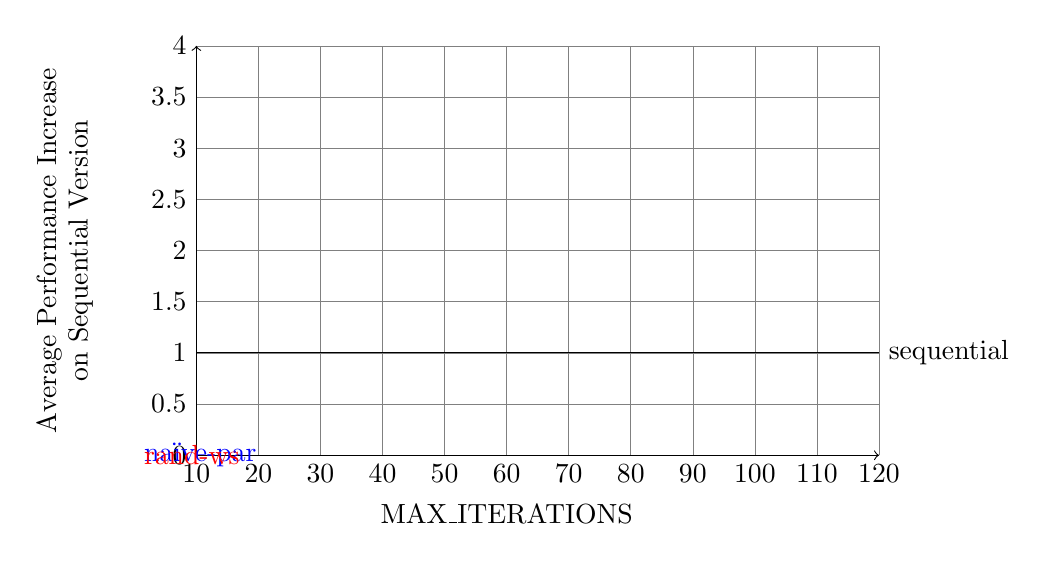
\begin{tikzpicture}[x=0.0065\textwidth,y=1.3cm]

  \def\xmin{10}
  \def\xmax{120}
  \def\ymin{0}
  \def\ymax{4}

  % grid
  \draw[style=help lines, ystep=0.5, xstep=10] (\xmin,\ymin) grid
  (\xmax,\ymax);

  % axes
  \draw[->] (\xmin,\ymin) -- (\xmax,\ymin); % node[right] {$x$};
  \draw[->] (\xmin,\ymin) -- (\xmin,\ymax); % node[above] {$y$};

  %labels      
    \draw (60,0) -- coordinate (x axis mid) (60,0);
	\draw (0,2) -- coordinate (y axis mid) (0,2);
    \node[below=0.5cm] at (x axis mid) {MAX\_ITERATIONS};
    \node[rotate=90, above=0.8cm] at (y axis mid) {Average Performance Increase};
    \node[rotate=90, above=0.4cm] at (y axis mid) {on Sequential Version};

  % xticks and yticks
  \foreach \x in {10,20,...,120}
    \node at (\x, \ymin) [below] {\x};
  \foreach \y in {0,0.5,1,...,4}
    \node at (\xmin,\y) [left] {\y};

    \draw[color=blue] plot[smooth,mark=*,mark size=0pt] file {results/pcworksize-np.data}
    node [right] {na\"{\i}ve-par};
    
    \draw[color=red] plot[smooth,mark=*,mark size=0pt] file {results/pcworksize-ws.data}
    node [right] {rand-ws};

    \draw[color=black] (\xmin,1) -- (\xmax,1) node[right] {sequential};

\end{tikzpicture}

% full caption
\caption{
    Average performance increase, relative to the sequential version of the program, against maximum number of iterations taken
    to determine the result of a single point. The raster-plane is ten-thousand squared in size for each sample.
}
\label{fig:perfworksizepc}
\end{figure}
